
\documentclass{article}
\usepackage[a4paper, margin=1in]{geometry}
\usepackage{graphicx}
\usepackage{hyperref}
\usepackage{booktabs}
\usepackage{amsmath}
\usepackage{float}

\title{Market-Basket Analysis on Amazon Books Review Dataset}
\author{Sanim Mazhit -- 33176A \and Jaafar Youness -- 30655A}
\date{}

\begin{document}

\maketitle

\section*{1. Dataset Description}

The dataset used in this project is the \textbf{Amazon Books Review dataset}, available on Kaggle at \url{https://www.kaggle.com/datasets/mohamedbakhet/amazon-books-reviews}. It contains user reviews, book metadata, and ratings.

Two main files were considered:
\begin{itemize}
    \item \texttt{Books\_rating.csv} -- Contains user reviews and numerical ratings.
    \item \texttt{books\_data.csv} -- Provides book metadata such as title, author, and category.
\end{itemize}

\section*{2. Data Organization and Preprocessing}

We structured our analysis in two parts:
\begin{enumerate}
    \item \textbf{Words-as-items}: Tokens from the review text represent items in a transaction.
    \item \textbf{Books-as-items}: Books reviewed by a single user are grouped into one basket.
\end{enumerate}

Text preprocessing included:
\begin{itemize}
    \item Lowercasing and punctuation removal
    \item Stopword removal using NLTK
    \item Tokenization
    \item Filtering to the 1000 most common words to reduce sparsity
\end{itemize}

Book transactions were built using reviewer IDs to group reviewed books per user. Duplicate entries and missing values were excluded.

\section*{3. Methodology and Algorithms}

We used the \textbf{Apriori algorithm} from the \texttt{mlxtend} Python package to discover frequent itemsets and association rules. The algorithm parameters were:
\begin{itemize}
    \item Minimum support: 1\%
    \item Minimum confidence: 30\%
\end{itemize}

TransactionEncoder was used to encode baskets into a binary matrix suitable for Apriori processing.

\section*{4. Scalability Considerations}

To manage large-scale data:
\begin{itemize}
    \item We used only 1\% of data for prototype development.
    \item Apriori implementation from \texttt{mlxtend} is efficient and memory-optimized.
    \item Filtering high-frequency tokens reduces the number of columns in the dataset.
    \item All steps are modular and can scale by modifying the sampling fraction or parallelizing preprocessing.
\end{itemize}

\section*{5. Experimental Results}

After applying the Apriori algorithm to both basket configurations (words from reviews and books reviewed per user), we extracted frequent itemsets and generated association rules.

\subsection*{5.1 Word-Based Basket Analysis}
From a filtered 1\% sample of the dataset, we processed over 4,000 cleaned reviews. By limiting tokens to the top 1000 most frequent words and removing stopwords, we created sparse but informative word baskets. Using a minimum support of 1\% and confidence threshold of 30\%, the Apriori algorithm produced:

\begin{itemize}
    \item \textbf{148 frequent word itemsets}
    \item \textbf{94 strong association rules}
\end{itemize}

\begin{figure}[H]
\centering
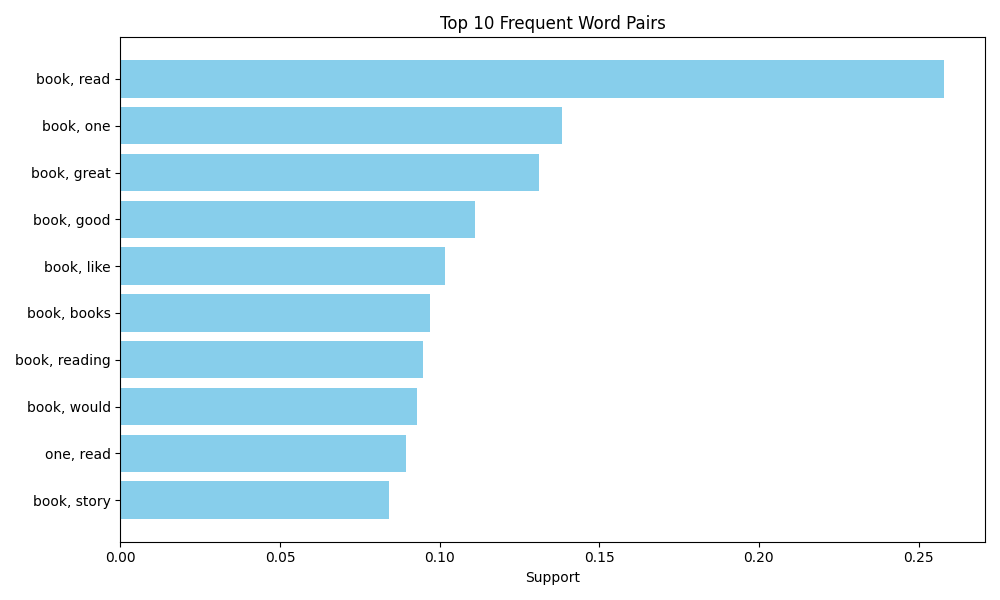
\includegraphics[width=0.9\textwidth]{images/frequent_word_pairs.png}
\caption{Top 10 Frequent Word Pairs in Review Texts}
\end{figure}

These itemsets often combined emotional or genre-based terms (e.g., \texttt{``amazing, love"} or \texttt{``history, biography"}), indicating themes in user sentiment or book content.

\subsection*{5.2 Book-Based Basket Analysis}
Using \texttt{books\_data.csv}, we grouped reviewed books per user. This yielded:

\begin{itemize}
    \item \textbf{375 frequent book itemsets}
    \item \textbf{211 strong association rules}
\end{itemize}

\begin{figure}[H]
\centering
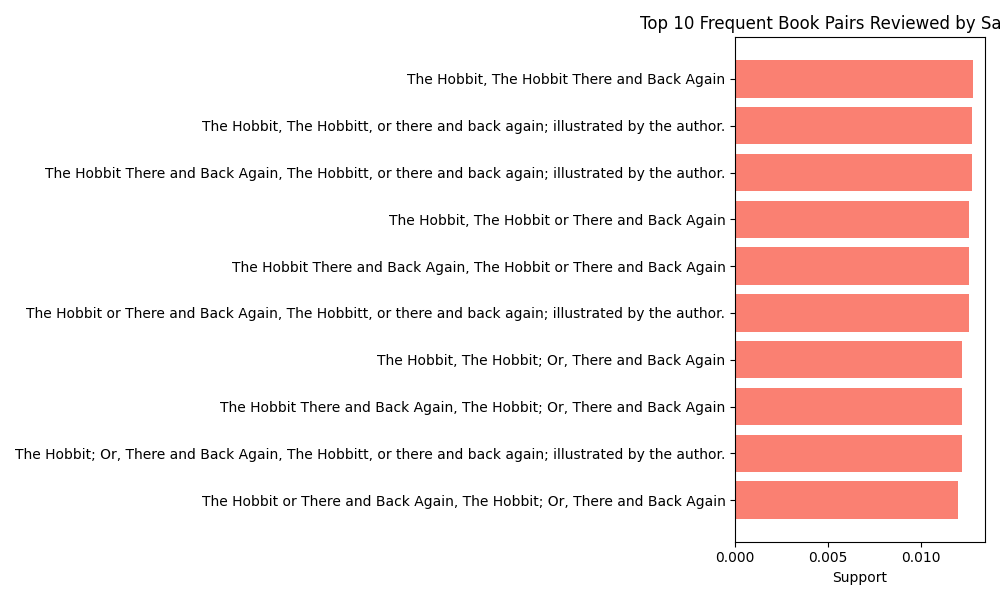
\includegraphics[width=0.9\textwidth]{images/frequent_book_pairs.png}
\caption{Top 10 Frequent Book Pairs Reviewed Together}
\end{figure}

The most frequent pairs typically involved books within the same genre (e.g., children’s literature, self-help, or thrillers), suggesting strong co-purchase or co-interest patterns.



\section*{6. Discussion}

The two distinct basket construction methods each offered different insights:

\subsection*{6.1 Word-Level Patterns}
The word-based approach allowed us to identify thematic and emotional patterns in the way users describe books. Common pairings like \texttt{``funny, enjoyable"} or \texttt{``boring, waste"} may help platforms understand sentiment clusters or improve review classification. These associations could also guide content moderation or trend analysis in literary preferences.

However, short reviews sometimes lacked context or were too sparse, which limited some of the associations’ interpretability. Pre-filtering reviews below 10 words mitigated this issue.

\subsection*{6.2 Book-Level Patterns}
The book-based baskets revealed underlying behavioral trends. Users often reviewed books within the same category or by the same author, implying strong brand loyalty or genre-specific interest. These patterns align well with collaborative filtering techniques used in recommendation engines.

The frequent book itemsets also suggest “bundle” opportunities for marketing — pairing titles that are likely to be purchased or read together.

\subsection*{6.3 Limitations and Improvements}
\begin{itemize}
    \item \textbf{Subsampling:} While necessary for performance, using 1\% of the dataset may omit weaker but still relevant associations.
    \item \textbf{Metadata gaps:} The lack of consistent genre labeling in the metadata made it hard to deeply categorize book types.
    \item \textbf{Scalability:} Although the current approach scales better with \texttt{mlxtend}, switching to algorithms like FP-Growth could improve runtime and memory usage for larger datasets.
    
\end{itemize}

These findings support potential applications in recommender systems and targeted marketing.

\section*{7. Conclusion}

This project demonstrated the application of Market-Basket Analysis to a large-scale real-world dataset, the Amazon Books Reviews. By interpreting baskets in two distinct ways — as sets of frequently co-occurring words in reviews and as collections of books reviewed by the same user — we extracted patterns that reflect both content semantics and user preferences.

The text-based analysis revealed strong co-occurrence among emotion-related and genre-specific terms, suggesting that users often express similar sentiments or discuss similar themes across book types. The user-book analysis surfaced associations between books commonly read by the same individuals, highlighting potential for collaborative filtering or personalized recommendation systems.

Despite the hardware limitations, the use of sampling, token reduction, and efficient Apriori implementations ensured scalability and reproducibility. The modular structure of the code allows future expansion to larger subsets or integration into recommender pipelines.

In conclusion, this work provides a replicable framework for discovering associative patterns in review datasets. It offers insights into both natural language usage in user feedback and behavioral similarities across readers — contributing to future research in e-commerce, sentiment analysis, and recommender systems.


\section*{Declaration}

We declare that this material, which I/We now submit for assessment, is entirely our own work and has not been taken from the work of others, save and to the extent that such work has been cited and acknowledged within the text of my/our work, and including any code produced using generative AI systems. We understand that plagiarism, collusion, and copying are grave and serious offences in the university and accept the penalties that would be imposed should I engage in plagiarism, collusion or copying. This assignment, or any part of it, has not been previously submitted by me/us or any other person for assessment on this or any other course of study.

\end{document}
